
The average person spends ninety-thousand hours at work \cite{90hours}. For office workers, their work environment is vital to their overall health and well-being. This project aims to develop software for a device that improves the well-being of employees and the ergonomics of office spaces. The project attempted to deliver an indoor mapping system through the use of audio technology.\\

Ergonomics is the study of optimising the work environment to encompass the requirements of the workers there best. The increase of ergonomics in an office space can be correlated to healthier and more productive workers, benefiting all parties. Ergonomics reduces the chances of workplace injury and can help improve employee morale. This, in turn, results in better production and more wealth for the employee. Critical elements of ergonomic office design are the equipment/furniture of the office, the layout and the environmental factors present (such as sound and temperature) \cite{ergonomics}.\\

A large component of ergonomics is the collection of information. Characterising the office environment is an important step in improving it. Information like temperature, humidity, noise levels, light exposure are all important when it comes to optimizing the office. Another example is indoor positioning data. This data will enable employers to know where desks are commonly positioned and where the popular areas within an office are. By studying the factors present in these region the office as a whole can be improved by emulating the factors that make said region popular. \\

This project into indoor mapping via sound will help companies and their employees, aiding Wellnomics, the University of Canterbury, and most importantly, the group. Wellnomics is a Christchurch based company that is a world leader in ergonomics. Wellnomics develops products to improve the health of employees across the world. Their software is used in a multitude of products that enable businesses to optimise their office environments. Wellnomics will benefit from this project as it has the potential to develop a feature that can be packaged in a device that can be included in hundreds of thousands of desks.\\

This project also enables engineering students to develop real-world design skills, preparing them for their actual jobs. It forces students to work professionally and understand design thinking. By having regular meetings, presenting findings and setting tasks, students advance their knowledge of engineering procedure and become better engineers.\\
\pagebreak
\subsection{User Requirements}

The user requirements outline what the project must achieve. These are the initial conditions that must be met for the project to be a success. The project aims to produce software designs and hardware recommendations towards integrating a new 3D mapping feature in the already developed LIMPET. The LIMPET is a Wellnomics design that collects data on various factors around an office. The design for it can be seen below in figure \ref{fig:limpet}. \\

\begin{figure}[H]
\centering
\noindent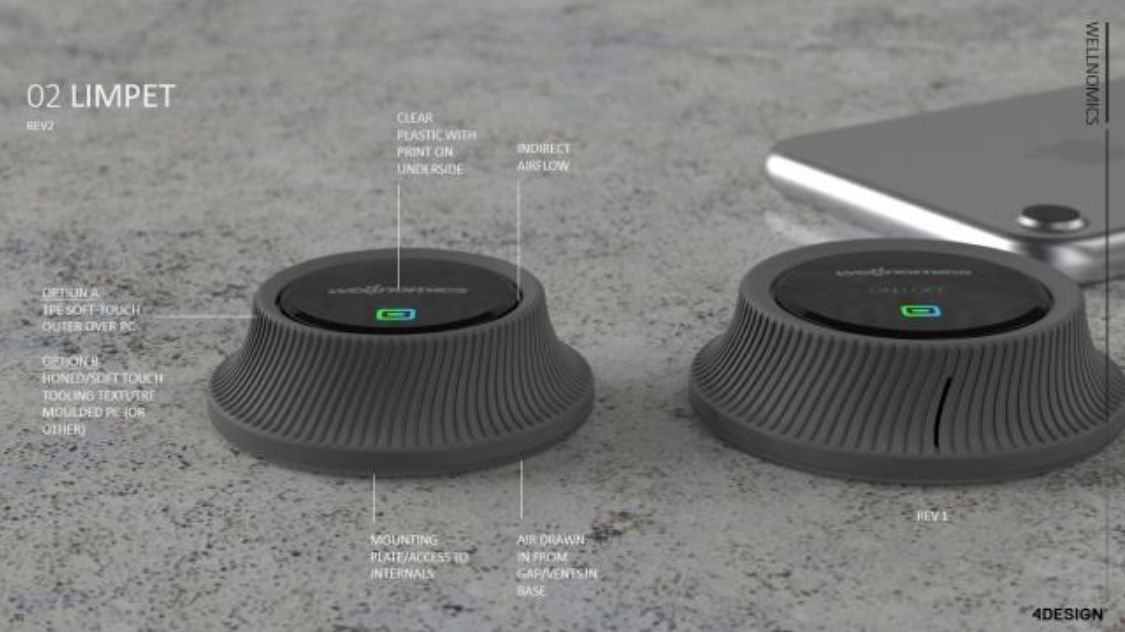
\includegraphics[width=10.26cm,height=5cm]{./images/limpet.png}
\caption{LIMPET design}
\label{fig:limpet}
\end{figure}

The LIMPET is designed to placed on desks and office furniture and continuously collect data throughout the day. It collects temperature, humidity, desk height and other data that impacts the well-being of the user. The aim is to add positioning functionality so that each LIMPETs position can be found in relation to other LIMPETs. The user requirements to achieve this are outlined below in The are summarised below in table \ref{tab:user_requirements}. 
\begin{center}
    \begin{table}[H]
    \captionsetup{singlelinecheck = false, format= hang, justification=raggedright, font=footnotesize, labelsep=space}
    \caption{User Requirements}
    \begin{adjustbox}{max width=\textwidth}
    \begin{tabular}{p{5.5cm}p{10.99cm}}
    \hline
    \multicolumn{1}{|p{5.5cm}}{Requirement} & 
    \multicolumn{1}{|p{10.99cm}|}{Description} \\ 
    \hline
    \multicolumn{1}{|p{5.5cm}}{Measure distance } & 
    \multicolumn{1}{|p{10.99cm}|}{Various methods can be used to achieve this. The measurements taken are essential to the mapping of the room.} \\ 
    \hline
    \multicolumn{1}{|p{5.5cm}}{Build a model to estimate positions accurately} & 
    \multicolumn{1}{|p{10.99cm}|}{Using measured distances, a mapping system must be created to accurately position devices.} \\ 
    \hline
    \multicolumn{1}{|p{5.5cm}}{Low cost} & 
    \multicolumn{1}{|p{10.99cm}|}{The aim is to produce a low cost system, as the LIMPET overall is a low cost solution. } \\ 
    \hline
    \multicolumn{1}{|p{5.5cm}}{Low power requirement} & 
    \multicolumn{1}{|p{10.99cm}|}{The LIMPET only has a certain amount of available power, and so the hardware used for this design cannot draw too much of this power.} \\ 
    \hline
    \multicolumn{1}{|p{5.5cm}}{Small design } & 
    \multicolumn{1}{|p{10.99cm}|}{The LIMPET is small device and as such cannot house large hardware. The hardware chosen for this project must be small enough to fit into the LIMPET. } \\ 
    \hline
    \multicolumn{1}{|p{5.5cm}}{Robustness to noise} & 
    \multicolumn{1}{|p{10.99cm}|}{The applicable environment may be noise rich and as such the method of communication must be considerate of this.} \\ 
    \hline
    \end{tabular}
    \end{adjustbox}
    \label{tab:user_requirements}\end{table}
\end{center}
\pagebreak
\subsection{Specifications}

The specifications outline what the final product will look like and how it fulfils the user requirements. They are summarised below in table \ref{tab:specifications}.
\begin{center}
    \begin{table}[H]
    \captionsetup{singlelinecheck = false, format= hang, justification=raggedright, font=footnotesize, labelsep=space}
    \caption{Specifications}
    \begin{adjustbox}{max width=\textwidth}
    \begin{tabular}{p{5.24cm}p{11.25cm}}
    \hline
    \multicolumn{1}{|p{5.24cm}}{Specifications} & 
    \multicolumn{1}{|p{11.25cm}|}{Description} \\ 
    \hline
    \multicolumn{1}{|p{5.24cm}}{Measuring distance using Audio signals. } & 
    \multicolumn{1}{|p{11.25cm}|}{The functionality for this specification could not be completed. The framework for achieving this is in place.} \\ 
    \hline
    \multicolumn{1}{|p{5.24cm}}{Positioning using 3D mesh } & 
    \multicolumn{1}{|p{11.25cm}|}{A system has been prototyped which can take in distance measurements and output a 3D map.} \\ 
    \hline
    \multicolumn{1}{|p{5.24cm}}{Frequency of Sound} & 
    \multicolumn{1}{|p{11.25cm}|}{To mitigate the impact of noise and attenuation, the transmitted wave can be between 1.6 kHz and 10 kHz, depending on the target environment.} \\ 
    \hline
    \multicolumn{1}{|p{5.24cm}}{MEMs Microphone } & 
    \multicolumn{1}{|p{11.25cm}|}{A small digital I2S MEMs microphone, SPH0644LM4H-B, is used. These are small, power-efficient and cheap.} \\ 
    \hline
    \multicolumn{1}{|p{5.24cm}}{Versatile Speaker} & 
    \multicolumn{1}{|p{11.25cm}|}{The AS01508MS-SP11-WP-R speaker is capable of delivering sounds between 600 Hz 20 kHz and is successfully programmed to do so.} \\ 
    \hline
    \end{tabular}
    \end{adjustbox}
    \label{tab:specifications}\end{table}
\end{center}

\subsection{Project Split}

The project naturally splits into four sections, The microphone, speaker, sound and the 3D mesh. Each part has equal importance as they are all required for the completion of the project. The sound decides what sort of signal is sent. This signal must be equipped to mitigate attenuation and noise and be reliably transmitted over a distance. The speaker must be driven with the correct input to produce the ideal signal. The proper amplifier must be constructed and tested for this. Similarly, on the other side, the microphone output must be processed and turned into reliable data. Finally, the distance data gained must be turned into 3d mesh. The individual break-up of these sections among group memebers is as follows:
\begin{itemize}
\item Aryan Srivastava - Sound
\item Laurence Prins - Speaker
\item Bill Liu - Microphone 
\item Toby Bourke - 3D Mesh 
\end{itemize}

